% SLH-DSA (FIPS 205): signing and verification, step by step.
% Build: tectonic slh-dsa-sign-verify.tex
% Every value in the running example is produced by `cargo run --example running_example`
% and re-derived by trace.py (a separate Python implementation of FIPS 205), see README.md.

\documentclass[aspectratio=169,11pt]{beamer}

\usepackage[T1]{fontenc}
\usepackage{lmodern}
\usepackage{booktabs}
\usepackage{array}
\usepackage{tikz}
\usetikzlibrary{arrows.meta,positioning,calc,decorations.pathreplacing,fit,shapes.misc}

% ---------------------------------------------------------------- look
\setbeamertemplate{navigation symbols}{}
\setbeamertemplate{footline}[frame number]
\setbeamertemplate{itemize items}[circle]
\definecolor{ink}{HTML}{1F2933}
\definecolor{secret}{HTML}{B42318}
\definecolor{pub}{HTML}{1D4ED8}
\definecolor{sig}{HTML}{047857}
\definecolor{accent}{HTML}{C2410C}
\definecolor{quiet}{HTML}{6B7280}
\definecolor{faint}{HTML}{E5E7EB}
\setbeamercolor{frametitle}{fg=ink}
\setbeamercolor{title}{fg=ink}
\setbeamercolor{structure}{fg=pub}
\setbeamercolor{normal text}{fg=ink}
\setbeamerfont{frametitle}{series=\bfseries,size=\Large}
\setbeamercolor{block title}{bg=faint,fg=ink}
\setbeamercolor{block body}{bg=faint!40}

\newcommand{\cat}{\mathbin{\Vert}}
\newcommand{\hx}[1]{\texttt{#1}}
\newcommand{\sk}[1]{\textcolor{secret}{#1}}
\newcommand{\pk}[1]{\textcolor{pub}{#1}}
\newcommand{\sg}[1]{\textcolor{sig}{#1}}
\newcommand{\alg}[1]{\textcolor{quiet}{\footnotesize[FIPS 205, Alg.~#1]}}
\newcommand{\step}[2]{\textcolor{accent}{\textbf{#1}}\enspace #2}

\tikzset{
  box/.style={draw=ink!60, rounded corners=3pt, minimum height=7mm, inner sep=3pt, font=\small},
  arr/.style={-{Latex[length=2mm]}, ink!70, thick},
  node/.style={circle, draw=ink!60, minimum size=5mm, inner sep=0pt, font=\scriptsize},
  leaf/.style={rectangle, rounded corners=1.5pt, draw=ink!60, minimum width=6mm, minimum height=5mm, inner sep=0pt, font=\scriptsize},
  hl/.style={fill=sig!18, draw=sig, thick},
  au/.style={fill=accent!18, draw=accent, thick},
  path/.style={draw=pub, very thick},
}

\title{SLH-DSA, Step by Step}
\subtitle{Signing and verification in FIPS 205, traced on a real signature}
\author{V-k-h}
\date{October 2026}

\begin{document}

% ================================================================ opening
\begin{frame}
  \titlepage
  \centering\footnotesize\textcolor{quiet}{Values from \texttt{slhsig} (github.com/V-k-h/slhsig), re-derived by a separate Python implementation}
\end{frame}

\begin{frame}{What this deck does}
  \begin{itemize}
    \item Walks through \textbf{pure SLH-DSA signing} (FIPS 205 Alg.~22, 19) and \textbf{verification} (Alg.~24, 20), one step per slide.
    \item Uses one running example, \textbf{SLH-DSA-SHAKE-128f}, with every intermediate value shown.
    \item The values are real: \texttt{slhsig} produced the signature, and a separate Python implementation of FIPS 205 re-derived the key, re-signed byte for byte, and verified.
  \end{itemize}
  \vspace{4mm}
  \textbf{Colour code:}\quad \sk{secret}\quad \pk{public}\quad \sg{signature bytes}\quad \textcolor{accent}{step / highlight}
\end{frame}

\begin{frame}{Running example: SLH-DSA-SHAKE-128f}
  \begin{columns}[T]
    \column{0.48\textwidth}
    \centering
    \begin{tabular}{@{}l l r@{}}
      \toprule
      Symbol & Meaning & Value \\
      \midrule
      $n$ & hash output (bytes) & 16 \\
      $h$ & hypertree height & 66 \\
      $d$ & hypertree layers & 22 \\
      $h'=h/d$ & XMSS tree height & 3 \\
      $a$ & FORS tree height & 6 \\
      $k$ & FORS trees & 33 \\
      $\lg w$ & Winternitz bits & 4 \\
      $\mathit{len}=2n+3$ & WOTS$^+$ chains & 35 \\
      $m$ & digest bytes & 34 \\
      \bottomrule
    \end{tabular}
    \column{0.48\textwidth}
    \begin{itemize}\small
      \item Security category 1; ``f'' = fast signing, larger signatures.
      \item Public key $2n = 32$ bytes, secret key $4n = 64$ bytes.
      \item Signature $(1 + k(1+a) + h + d\cdot\mathit{len})\cdot n$ $= 17{,}088$ bytes.
      \item Every hash is SHAKE256 truncated to the stated length (Section 11.1).
    \end{itemize}
  \end{columns}
\end{frame}

\begin{frame}{Keys}
  \begin{columns}[T]
    \column{0.55\textwidth}
    \textbf{Secret key} \quad $\mathsf{SK} = \sk{\mathsf{SK.seed}} \cat \sk{\mathsf{SK.prf}} \cat \pk{\mathsf{PK.seed}} \cat \pk{\mathsf{PK.root}}$\\[2mm]
    \textbf{Public key} \quad $\mathsf{PK} = \pk{\mathsf{PK.seed}} \cat \pk{\mathsf{PK.root}}$\\[4mm]
    \begin{itemize}\small
      \item \sk{SK.seed} derives every WOTS$^+$ and FORS secret through PRF.
      \item \sk{SK.prf} keys the message randomizer $R$.
      \item \pk{PK.seed} separates this key's hashes from every other key's.
      \item \pk{PK.root} is the root of the single XMSS tree in the top layer.
    \end{itemize}
    \column{0.42\textwidth}
    \footnotesize
    \textbf{Example} (seeds chosen for readability):\\[1mm]
    \begin{tabular}{@{}l l@{}}
      \sk{SK.seed} & \hx{000102\ldots0e0f} \\
      \sk{SK.prf}  & \hx{101112\ldots1e1f} \\
      \pk{PK.seed} & \hx{202122\ldots2e2f} \\
      \pk{PK.root} & \hx{a90e4715b9a925c3}\\
                   & \hx{32801767fd786371}
    \end{tabular}\\[3mm]
    Key generation \alg{18}:\\[1mm]
    $\pk{\mathsf{PK.root}} = \texttt{xmss\_node}(\sk{\mathsf{SK.seed}}, 0, h',$\\
    \hspace*{12mm}$\pk{\mathsf{PK.seed}}, \mathsf{ADRS}_{\text{layer } 21})$
  \end{columns}
\end{frame}

\begin{frame}{The structure: a hypertree of XMSS trees over a FORS forest}
  \centering
  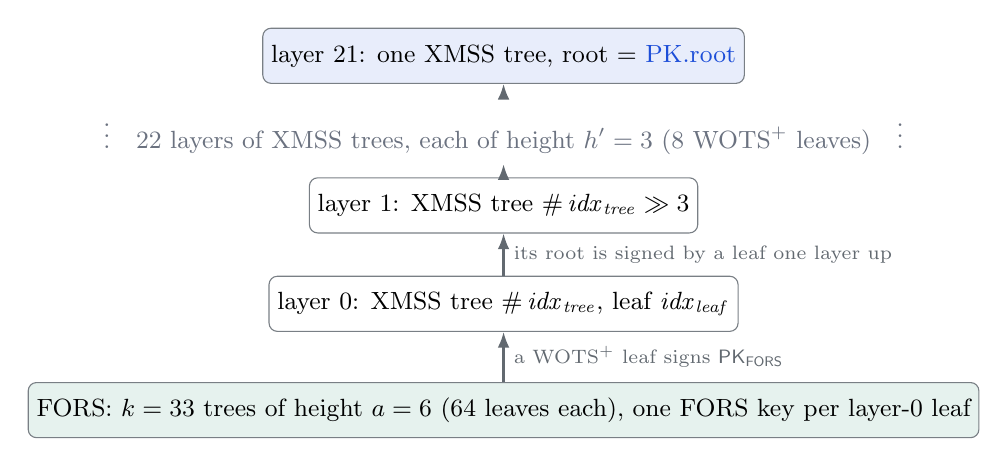
\begin{tikzpicture}[x=1cm,y=1cm]
    % top layer
    \node[box, fill=pub!10] (top) at (0,5.0) {layer 21: one XMSS tree, root $=$ \pk{PK.root}};
    \node[font=\small, quiet] (dots) at (0,4.05) {$\vdots$\quad 22 layers of XMSS trees, each of height $h'=3$ (8 WOTS$^+$ leaves)\quad$\vdots$};
    \node[box] (l1) at (0,3.1) {layer 1: XMSS tree $\#\,\mathit{idx}_{\mathit{tree}} \gg 3$};
    \node[box] (l0) at (0,1.85) {layer 0: XMSS tree $\#\,\mathit{idx}_{\mathit{tree}}$, leaf $\mathit{idx}_{\mathit{leaf}}$};
    \node[box, fill=sig!10, minimum width=11cm] (fors) at (0,0.5) {FORS: $k=33$ trees of height $a=6$ (64 leaves each), one FORS key per layer-0 leaf};
    \draw[arr] (fors) -- node[right, font=\scriptsize]{a WOTS$^+$ leaf signs $\mathsf{PK}_{\mathsf{FORS}}$} (l0);
    \draw[arr] (l0) -- node[right, font=\scriptsize]{its root is signed by a leaf one layer up} (l1);
    \draw[arr, dashed] (l1) -- (dots);
    \draw[arr, dashed] (dots) -- (top);
  \end{tikzpicture}
  \vspace{2mm}

  \small The message picks one of $2^{63} \times 8 = 2^{66}$ FORS keys (few-time). That FORS public key is certified by a chain of one-time WOTS$^+$ signatures up to \pk{PK.root}.
\end{frame}

\begin{frame}{Tweakable hash functions (SHAKE instantiation)}
  \centering
  \renewcommand{\arraystretch}{1.25}
  \begin{tabular}{@{}l l l@{}}
    \toprule
    Function & SHAKE256 input, output length (Section 11.1) & Used for \\
    \midrule
    PRF & $\pk{\mathsf{PK.seed}} \cat \mathsf{ADRS} \cat \sk{\mathsf{SK.seed}}$, \ $n$ bytes & WOTS$^+$ and FORS secrets \\
    F & $\pk{\mathsf{PK.seed}} \cat \mathsf{ADRS} \cat M_1$, \ $n$ bytes & chain steps, FORS leaves \\
    H & $\pk{\mathsf{PK.seed}} \cat \mathsf{ADRS} \cat M_2$, \ $n$ bytes & Merkle nodes \\
    T$_\ell$ & $\pk{\mathsf{PK.seed}} \cat \mathsf{ADRS} \cat M_\ell$, \ $n$ bytes & compress $\ell$ nodes \\
    PRF$_{\mathsf{msg}}$ & $\sk{\mathsf{SK.prf}} \cat \mathit{opt\_rand} \cat M$, \ $n$ bytes & randomizer $R$ \\
    H$_{\mathsf{msg}}$ & $R \cat \pk{\mathsf{PK.seed}} \cat \pk{\mathsf{PK.root}} \cat M$, \ $m$ bytes & message digest \\
    \bottomrule
  \end{tabular}
  \vspace{3mm}

  \footnotesize\textcolor{quiet}{SHA2 sets use SHA-256 with a 22-byte compressed ADRS; categories 3 and 5 switch H, T$_\ell$, PRF$_{\mathsf{msg}}$ and H$_{\mathsf{msg}}$ to SHA-512 (Section 11.2).}
\end{frame}

\begin{frame}{The address ADRS: every hash call gets a unique 32-byte tweak}
  \centering
  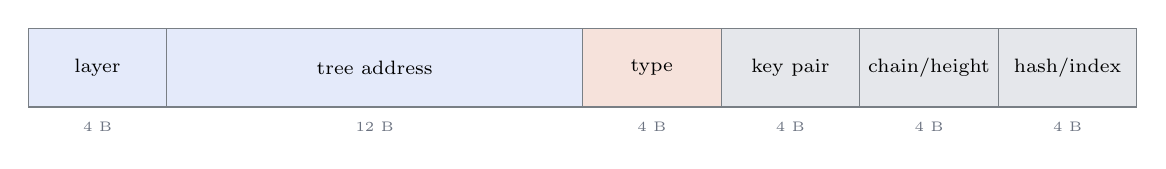
\begin{tikzpicture}[x=4.4mm,y=1cm]
    \foreach \x/\w/\lab/\col in {0/4/layer/pub!12, 4/12/tree address/pub!12, 16/4/type/accent!15, 20/4/key pair/faint, 24/4/chain\slash height/faint, 28/4/hash\slash index/faint}{
      \draw[fill=\col, draw=ink!60] (\x,0) rectangle ++(\w,1);
      \node[font=\scriptsize, align=center] at (\x+\w/2,0.5) {\lab};
      \node[font=\tiny, quiet] at (\x+\w/2,-0.25) {\w\ B};
    }
  \end{tikzpicture}
  \vspace{3mm}

  \small
  \begin{tabular}{@{}l l l@{}}
    \toprule
    Type & Hash it tweaks & Last 12 bytes \\
    \midrule
    0 \texttt{WOTS\_HASH}  & F in a WOTS$^+$ chain & key pair, chain, hash \\
    1 \texttt{WOTS\_PK}    & T$_{\mathit{len}}$ compressing a WOTS$^+$ public key & key pair \\
    2 \texttt{TREE}        & H for an XMSS Merkle node & height, index \\
    3 \texttt{FORS\_TREE}  & F, H inside a FORS tree & key pair, height, index \\
    4 \texttt{FORS\_ROOTS} & T$_k$ compressing the FORS roots & key pair \\
    5, 6 \texttt{*\_PRF}   & PRF deriving WOTS$^+$ / FORS secrets & as for 0 / 3 \\
    \bottomrule
  \end{tabular}
\end{frame}

% ================================================================ signing
\section{Signing}

\begin{frame}{Signing at a glance}
  \centering
  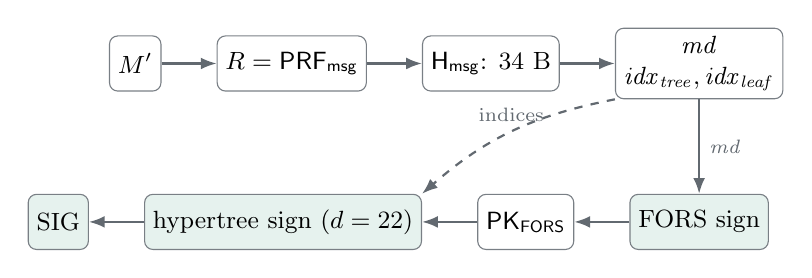
\begin{tikzpicture}[node distance=5mm and 7mm]
    \node[box] (m) {$M'$};
    \node[box, right=of m] (r) {$R=\mathsf{PRF_{msg}}$};
    \node[box, right=of r] (dg) {$\mathsf{H_{msg}}$: 34 B};
    \node[box, right=of dg, align=center] (sp) {$\mathit{md}$\\$\mathit{idx}_{\mathit{tree}}, \mathit{idx}_{\mathit{leaf}}$};
    \node[box, below=12mm of sp, fill=sig!10] (fs) {FORS sign};
    \node[box, left=of fs] (pf) {$\mathsf{PK}_{\mathsf{FORS}}$};
    \node[box, left=of pf, fill=sig!10] (ht) {hypertree sign ($d=22$)};
    \node[box, left=of ht, fill=sig!10] (out) {SIG};
    \draw[arr] (m) -- (r); \draw[arr] (r) -- (dg); \draw[arr] (dg) -- (sp);
    \draw[arr] (sp) -- node[right,font=\scriptsize]{$\mathit{md}$} (fs);
    \draw[arr] (fs) -- (pf); \draw[arr] (pf) -- (ht); \draw[arr] (ht) -- (out);
    \draw[arr, dashed] (sp.south west) to[bend right=15] node[above, font=\scriptsize]{indices} (ht.north east);
  \end{tikzpicture}
  \vspace{4mm}

  \small
  \begin{columns}[T]
    \column{0.45\textwidth}
    \begin{enumerate}
      \item Encode message and context: $M'$
      \item Randomize: $R$
      \item Hash: the 34-byte digest
      \item Split: FORS input, hypertree position
    \end{enumerate}
    \column{0.5\textwidth}
    \begin{enumerate}\setcounter{enumi}{4}
      \item FORS-sign $\mathit{md}$; recompute $\mathsf{PK}_{\mathsf{FORS}}$
      \item Hypertree-sign $\mathsf{PK}_{\mathsf{FORS}}$
      \item $\mathsf{SIG}=R\cat\mathsf{SIG_{FORS}}\cat\mathsf{SIG_{HT}}$
    \end{enumerate}
  \end{columns}
\end{frame}

\begin{frame}{Step 1: encode the message and context \alg{22}}
  \[ M' = \mathtt{toByte}(0,1) \cat \mathtt{toByte}(|\mathit{ctx}|, 1) \cat \mathit{ctx} \cat M \]
  \begin{itemize}
    \item The leading \hx{00} marks \emph{pure} signing; pre-hash signing uses \hx{01} plus the hash OID, so neither kind verifies as the other.
    \item The context string (at most 255 bytes) binds the signature to an application or protocol.
  \end{itemize}
  \vspace{2mm}
  \begin{block}{Example: $M = $ ``\texttt{Hello, FIPS 205!}'', $\mathit{ctx} = $ ``\texttt{slides}''}
    \centering\ttfamily
    \textcolor{accent}{00}\;\textcolor{accent}{06}\;\pk{736c69646573}\;48656c6c6f2c20464950532032303521\\[1mm]
    \sffamily\footnotesize \textcolor{accent}{pure, $|\mathit{ctx}|=6$}\quad \pk{``slides''}\quad ``Hello, FIPS 205!'' \quad (24 bytes)
  \end{block}
\end{frame}

\begin{frame}{Step 2: the randomizer $R$ \alg{19, lines 2--4}}
  \[ \sg{R} = \mathsf{PRF_{msg}}(\sk{\mathsf{SK.prf}}, \mathit{opt\_rand}, M') \]
  \begin{columns}[T]
    \column{0.5\textwidth}
    \begin{block}{Hedged (default)}\small
      $\mathit{opt\_rand}$ = $n$ fresh random bytes per signature. Two signatures of the same message differ, and side-channel traces never repeat.
    \end{block}
    \column{0.5\textwidth}
    \begin{block}{Deterministic}\small
      $\mathit{opt\_rand} = \pk{\mathsf{PK.seed}}$. The same message always yields the same signature. FIPS 205 asks that a key serve one variant only.
    \end{block}
  \end{columns}
  \vspace{3mm}
  \begin{itemize}\small
    \item $R$ is the first $n$ bytes of the signature, so it is public once signed.
    \item Example (deterministic): \sg{\hx{R = c739f8d2231214e790d9dc92032bc4fb}}
  \end{itemize}
\end{frame}

\begin{frame}{Step 3: the message digest \alg{19, line 5}}
  \[ \mathit{digest} = \mathsf{H_{msg}}(\sg{R}, \pk{\mathsf{PK.seed}}, \pk{\mathsf{PK.root}}, M') \qquad (m = 34 \text{ bytes}) \]
  \begin{itemize}
    \item Randomized hashing: $R$ is mixed in, so a collision on $\mathsf{H_{msg}}$ alone does not give a forgery.
    \item Binding \pk{PK.seed} and \pk{PK.root} ties the digest to this key.
    \item The verifier recomputes the same digest from public values: \emph{nothing derived from it is secret}.
  \end{itemize}
  \vspace{2mm}
  \begin{block}{Example}
    \centering\ttfamily\small
    4ecb576da7c253e0fa1460b299ada5e7b776449189723982f0\,5ac8de2436007947\,21
  \end{block}
\end{frame}

\begin{frame}{Step 4: split the digest \alg{19, lines 6--10}}
  \centering
  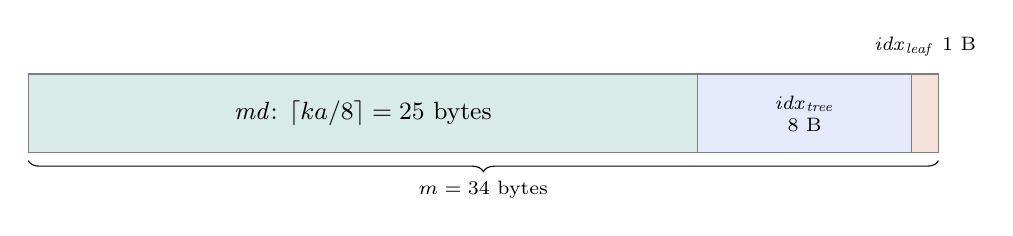
\begin{tikzpicture}[x=3.4mm,y=1cm]
    \draw[fill=sig!15, draw=ink!60] (0,0) rectangle (25,1);
    \node[font=\small] at (12.5,0.5) {$\mathit{md}$: $\lceil k a/8\rceil = 25$ bytes};
    \draw[fill=pub!12, draw=ink!60] (25,0) rectangle (33,1);
    \node[font=\scriptsize, align=center] at (29,0.5) {$\mathit{idx}_{\mathit{tree}}$\\8 B};
    \draw[fill=accent!15, draw=ink!60] (33,0) rectangle (34,1);
    \node[font=\scriptsize] at (33.5,1.35) {$\mathit{idx}_{\mathit{leaf}}$ 1 B};
    \draw[decorate, decoration={brace, mirror, amplitude=4pt}] (0,-0.1) -- (34,-0.1) node[midway, below=4pt, font=\scriptsize] {$m = 34$ bytes};
  \end{tikzpicture}
  \vspace{2mm}

  \small
  \begin{tabular}{@{}l l l@{}}
    \toprule
    Field & Rule & Example \\
    \midrule
    $\mathit{md}$ & first 25 bytes ($k \cdot a = 198$ bits used) & \hx{4ecb576d\ldots723982f0} \\
    $\mathit{idx}_{\mathit{tree}}$ & next 8 bytes, mod $2^{h-h'} = 2^{63}$ & \hx{0x5ac8de2436007947} (63 bits) \\
    $\mathit{idx}_{\mathit{leaf}}$ & next byte, mod $2^{h'} = 8$ & \hx{0x21} mod 8 $= 1$ \\
    \bottomrule
  \end{tabular}
  \vspace{3mm}

  \footnotesize\textcolor{quiet}{For the 256f sets $h - h' = 64$: an implementation computing $2^{64}$ in a 64-bit word overflows and pins every signature to tree 0.}
\end{frame}

\begin{frame}{Step 5: FORS indices from $\mathit{md}$ \alg{16, line 2}}
  \[ \mathit{indices} = \mathtt{base\_2b}(\mathit{md}, a, k) \qquad k = 33 \text{ indices of } a = 6 \text{ bits each} \]
  \centering
  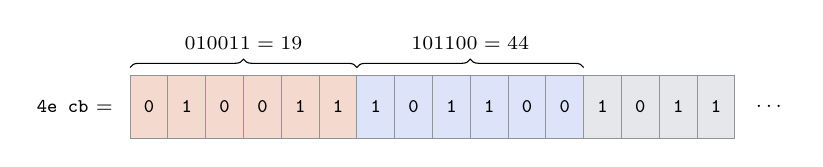
\begin{tikzpicture}[x=4.8mm]
    \foreach \b [count=\i from 0] in {0,1,0,0,1,1,1,0,1,1,0,0,1,0,1,1}{
      \ifnum\i<6 \def\c{accent!20}\else\ifnum\i<12 \def\c{pub!15}\else\def\c{faint}\fi\fi
      \draw[fill=\c, draw=ink!50] (\i,0) rectangle ++(1,0.8);
      \node[font=\scriptsize\ttfamily] at (\i+0.5,0.4) {\b};
    }
    \node[font=\scriptsize, anchor=east] at (-0.2,0.4) {\hx{4e cb} $=$};
    \draw[decorate, decoration={brace, amplitude=3pt}] (0,0.9) -- (6,0.9) node[midway, above=3pt, font=\scriptsize] {$010011 = 19$};
    \draw[decorate, decoration={brace, amplitude=3pt}] (6,0.9) -- (12,0.9) node[midway, above=3pt, font=\scriptsize] {$101100 = 44$};
    \node[font=\scriptsize, anchor=west] at (16.3,0.4) {\ldots};
  \end{tikzpicture}
  \vspace{3mm}

  \small
  All 33 indices in the example:\\[1mm]
  \ttfamily\footnotesize 19 44 45 23 27 26 31 2 20 62 3 58 5 6 2 50 38 26 54 37 57 59 29 54 17 9 6 9 28 35 38 2 60\\[2mm]
  \sffamily\small Index $i$ selects one of the 64 leaves of FORS tree $i$: global leaf $i\cdot 2^a + \mathit{indices}[i]$.
\end{frame}

\begin{frame}{Step 6: FORS signing, one tree \alg{14--16}}
  \begin{columns}[c]
    \column{0.52\textwidth}
    \centering
    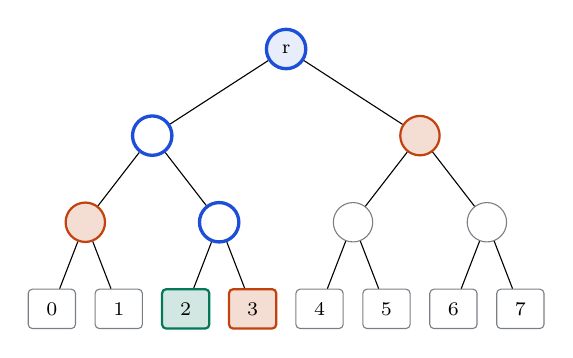
\begin{tikzpicture}[level distance=11mm, every node/.style={node},
        level 1/.style={sibling distance=34mm}, level 2/.style={sibling distance=17mm},
        level 3/.style={sibling distance=8.5mm}]
      % illustrative tree of height 3 (the real one has height a = 6)
      \node[path, fill=pub!10] (root) {r}
        child {node[path] {}
          child {node[au] {}
            child {node[leaf] {0}} child {node[leaf] {1}} }
          child {node[path] {}
            child {node[leaf, hl] {2}} child {node[leaf, au] {3}} } }
        child {node[au] {}
          child {node {} child {node[leaf] {4}} child {node[leaf] {5}} }
          child {node {} child {node[leaf] {6}} child {node[leaf] {7}} } };
    \end{tikzpicture}\\
    \footnotesize\textcolor{quiet}{Height 3 shown; the real trees have height $a=6$.}
    \column{0.46\textwidth}\small
    For tree $i$ with index $t = \mathit{indices}[i]$:
    \begin{enumerate}
      \item Reveal the \sg{leaf secret} at leaf $i\cdot 2^a + t$:\\
        $\sk{\mathit{sk}} = \mathsf{PRF}(\pk{\mathsf{PK.seed}}, \sk{\mathsf{SK.seed}}, \mathsf{ADRS})$, type \texttt{FORS\_PRF}.
      \item Add the \textcolor{accent}{authentication path}: the $a$ siblings on the way to the root.
    \end{enumerate}
    Leaves are $\mathsf{F}(\mathit{sk})$; inner nodes are $\mathsf{H}(\mathit{left}\cat\mathit{right})$.\\[2mm]
    \textbf{Example:} tree 0 reveals leaf 19; tree 1 reveals global leaf $64 + 44 = 108$.\\[2mm]
    $\mathsf{SIG_{FORS}} = k \times (\mathit{sk} \cat \mathit{auth}_{0..a-1})$ $= 33 \times 7 \times 16 = 3{,}696$ bytes.
  \end{columns}
\end{frame}

\begin{frame}{Step 6 (cont.): FORS public key \alg{17}}
  \[ \mathsf{PK}_{\mathsf{FORS}} = \mathsf{T}_k\bigl(\pk{\mathsf{PK.seed}}, \mathsf{ADRS_{FORS\_ROOTS}}, \mathit{root}_0 \cat \cdots \cat \mathit{root}_{32}\bigr) \]
  \begin{itemize}
    \item The signer recomputes each root from the signature it just produced (\texttt{fors\_pkFromSig}), exactly as a verifier will.
    \item All FORS addresses carry $\mathit{idx}_{\mathit{tree}}$ and key pair $\mathit{idx}_{\mathit{leaf}}$: each layer-0 leaf owns its own FORS key.
    \item FORS is \emph{few-time}: each use reveals 33 leaf secrets, and forgeries only become feasible after a key signs many messages. That is why $2^{66}$ instances exist.
  \end{itemize}
  \vspace{2mm}
  \begin{block}{Example}
    \footnotesize\ttfamily
    \begin{tabular}{@{}l l@{}}
      root$_0$ & 208e67d646a9fdc1f231b941eb65083c \\
      root$_1$ & 29ba73ed4c5292734aba1fad3f0b255b \\
      root$_2$ & 10e642d5b9806499c64832dc38de5480 \quad \sffamily\ldots\ (33 roots) \\
      \textbf{PK$_{\text{FORS}}$} & \textbf{0608a9a55575d3e4ed2b4b692f07fd67}
    \end{tabular}
  \end{block}
\end{frame}

\begin{frame}{Step 7: hypertree signing \alg{12}}
  \begin{columns}[T]
    \column{0.47\textwidth}\small
    \begin{enumerate}
      \item Layer 0: XMSS tree $\mathit{idx}_{\mathit{tree}}$, leaf $\mathit{idx}_{\mathit{leaf}}$ signs \pk{$\mathsf{PK}_{\mathsf{FORS}}$}.
      \item Recompute that tree's root from the new signature.
      \item Move up: \\
        $\mathit{idx}_{\mathit{leaf}} \gets \mathit{idx}_{\mathit{tree}} \bmod 2^{h'}$ \\
        $\mathit{idx}_{\mathit{tree}} \gets \mathit{idx}_{\mathit{tree}} \gg h'$
      \item Layer $j$ signs the root of layer $j-1$. Repeat to layer $d-1 = 21$.
    \end{enumerate}
    \vspace{1mm}
    $\mathsf{SIG_{HT}} = 22 \times (\mathit{len} + h')\cdot n = 22 \times 608 = 13{,}376$ bytes.
    \column{0.5\textwidth}
    \centering\footnotesize
    \begin{tabular}{@{}r r r@{}}
      \toprule
      layer & $\mathit{idx}_{\mathit{tree}}$ & $\mathit{idx}_{\mathit{leaf}}$ \\
      \midrule
      0 & 6541722705861835079 & 1 \\
      1 & 817715338232729384 & 7 \\
      2 & 102214417279091173 & 0 \\
      3 & 12776802159886396 & 5 \\
      $\vdots$ & $\vdots$ & $\vdots$ \\
      20 & 5 & 5 \\
      21 & 0 & 5 \\
      \bottomrule
    \end{tabular}\\[1mm]
    \textcolor{quiet}{Each step drops 3 bits of $\mathit{idx}_{\mathit{tree}}$: $63 = 21 \times 3$, so layer 21 is tree 0.}
  \end{columns}
\end{frame}

\begin{frame}{Step 7a: WOTS$^+$ message digits and checksum \alg{7, lines 1--7}}
  The $n$-byte message (here \pk{$\mathsf{PK}_{\mathsf{FORS}}$}) becomes $\mathit{len} = 35$ base-16 digits:
  \begin{itemize}
    \item $\mathit{len}_1 = 32$ digits: the nibbles of the message.
    \item $\mathit{len}_2 = 3$ digits: the checksum $\sum_i (15 - \mathit{msg}[i])$, shifted left 4 bits and written as two bytes.
  \end{itemize}
  \vspace{2mm}
  \begin{block}{Example: \hx{0608a9a55575d3e4ed2b4b692f07fd67}}
    \footnotesize
    \ttfamily 0 6 0 8 10 9 10 5 5 5 7 5 13 3 14 4 14 13 2 11 4 11 6 9 2 15 0 7 15 13 6 7 \;\textcolor{accent}{| 0 15 1}\\[1mm]
    \sffamily Digit sum $= 239$; checksum $= 32\cdot 15 - 239 = 241$; $241 \ll 4 = 3856 = \hx{0x0F10}$ $\Rightarrow$ \textcolor{accent}{0, 15, 1}.
  \end{block}
  \vspace{1mm}
  \small\textbf{Why the checksum:} raising any message digit lowers the checksum. A forger who wants to sign a larger digit would have to move a checksum chain \emph{backwards}, which means inverting F.
\end{frame}

\begin{frame}{Step 7b: WOTS$^+$ chains \alg{5, 7}}
  \centering
  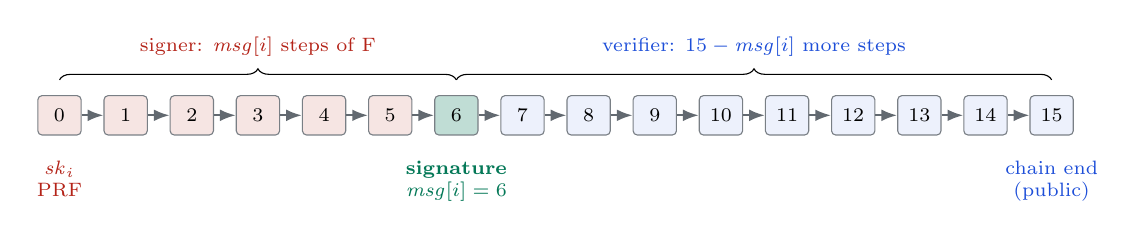
\begin{tikzpicture}[x=8.4mm]
    \foreach \i in {0,...,15}{
      \ifnum\i<6 \def\fillc{secret!12}\else\ifnum\i=6 \def\fillc{sig!25}\else\def\fillc{pub!8}\fi\fi
      \node[leaf, minimum width=5.5mm, fill=\fillc] (c\i) at (\i,0) {\i};
    }
    \foreach \i [evaluate=\i as \j using int(\i+1)] in {0,...,14}{ \draw[arr] (c\i) -- (c\j); }
    \node[font=\scriptsize, secret, below=2mm of c0, align=center] {$\mathit{sk}_i$\\PRF};
    \node[font=\scriptsize, sig, below=2mm of c6, align=center] {\textbf{signature}\\$\mathit{msg}[i]=6$};
    \node[font=\scriptsize, pub, below=2mm of c15, align=center] {chain end\\(public)};
    \draw[decorate, decoration={brace, amplitude=4pt}] (0,0.45) -- (6,0.45) node[midway, above=5pt, font=\scriptsize, secret] {signer: $\mathit{msg}[i]$ steps of F};
    \draw[decorate, decoration={brace, amplitude=4pt}] (6,0.45) -- (15,0.45) node[midway, above=5pt, font=\scriptsize, pub] {verifier: $15 - \mathit{msg}[i]$ more steps};
  \end{tikzpicture}
  \vspace{4mm}

  \small
  \begin{itemize}
    \item Chain $i$ starts at $\sk{\mathit{sk}_i} = \mathsf{PRF}(\pk{\mathsf{PK.seed}}, \sk{\mathsf{SK.seed}}, \mathsf{ADRS_{WOTS\_PRF}})$ and steps with $\mathsf{F}$, the hash address counting the step.
    \item Signature element $i$ is the chain value after $\mathit{msg}[i]$ steps (chain 1 of the example has $\mathit{msg}[1]=6$, as drawn).
    \item The public key is $\mathsf{T}_{35}$ over the 35 chain ends; it is never stored, only recomputed.
  \end{itemize}
\end{frame}

\begin{frame}{Step 7c: XMSS signature and auth path \alg{9--10}}
  \begin{columns}[c]
    \column{0.5\textwidth}
    \centering
    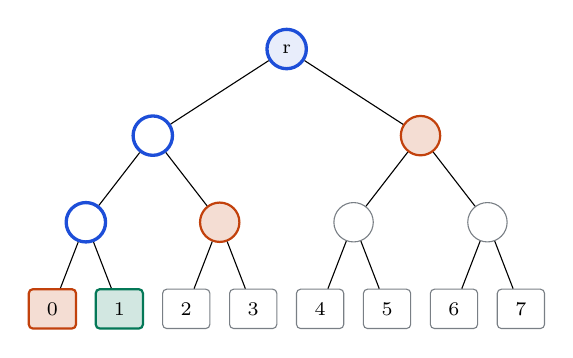
\begin{tikzpicture}[level distance=11mm, every node/.style={node},
        level 1/.style={sibling distance=34mm}, level 2/.style={sibling distance=17mm},
        level 3/.style={sibling distance=8.5mm}]
      \node[path, fill=pub!10] {r}
        child {node[path] {}
          child {node[path] {} child {node[leaf, au] {0}} child {node[leaf, hl] {1}} }
          child {node[au] {} child {node[leaf] {2}} child {node[leaf] {3}} } }
        child {node[au] {}
          child {node {} child {node[leaf] {4}} child {node[leaf] {5}} }
          child {node {} child {node[leaf] {6}} child {node[leaf] {7}} } };
    \end{tikzpicture}\\
    \footnotesize\textcolor{quiet}{Layer 0 of the example: $h'=3$, leaf $\mathit{idx}_{\mathit{leaf}}=1$.}
    \column{0.48\textwidth}\small
    \textbf{XMSS signature} $=$ \sg{WOTS$^+$ signature} (35 nodes) $\cat$ \textcolor{accent}{auth path} (3 nodes) $= 608$ bytes.\\[2mm]
    Auth node $j$ is \texttt{xmss\_node} at height $j$, index $(\mathit{idx}\gg j)\oplus 1$:
    \begin{itemize}
      \item $j=0$: leaf 0, one WOTS$^+$ public key
      \item $j=1$: node over leaves 2--3
      \item $j=2$: node over leaves 4--7
    \end{itemize}
    So each XMSS signature recomputes 7 of the tree's 8 WOTS$^+$ public keys (35 chains of 15 steps each).
    This is where signing time goes.
  \end{columns}
\end{frame}

\begin{frame}{Step 8: assemble the signature \alg{19, lines 15--18}}
  \centering
  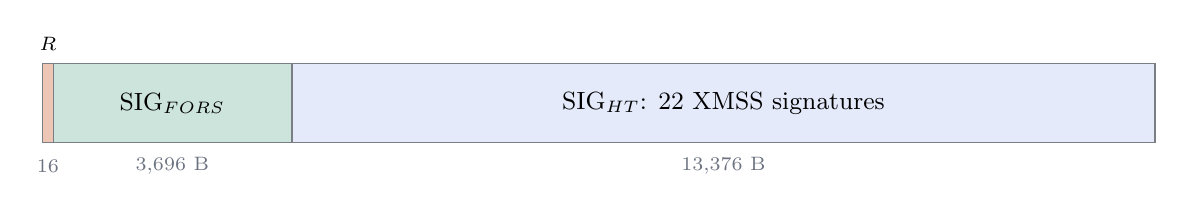
\begin{tikzpicture}[x=1mm,y=1cm]
    % Widths proportional to 16 | 3,696 | 13,376 bytes over 140 mm; R is widened to stay visible.
    \draw[fill=accent!30, draw=ink!60] (0,0) rectangle (1.4,1);
    \draw[fill=sig!20, draw=ink!60] (1.4,0) rectangle (31.7,1);
    \node[font=\small] at (16.5,0.5) {SIG$_{\text{FORS}}$};
    \draw[fill=pub!12, draw=ink!60] (31.7,0) rectangle (141.3,1);
    \node[font=\small] at (86.5,0.5) {SIG$_{\text{HT}}$: 22 XMSS signatures};
    \node[font=\scriptsize, anchor=south] at (0.7,1.05) {$R$};
    \node[font=\scriptsize, quiet] at (0.7,-0.3) {16};
    \node[font=\scriptsize, quiet] at (16.5,-0.3) {3,696 B};
    \node[font=\scriptsize, quiet] at (86.5,-0.3) {13,376 B};
  \end{tikzpicture}
  \vspace{4mm}

  \[ \mathsf{SIG} = \sg{R} \cat \sg{\mathsf{SIG_{FORS}}} \cat \sg{\mathsf{SIG_{HT}}} \qquad 16 + 3{,}696 + 13{,}376 = 17{,}088 \text{ bytes} \]
  \small
  \begin{itemize}
    \item Byte offsets: $R$ at 0, SIG$_{\text{FORS}}$ at 16, SIG$_{\text{HT}}$ at 3,712; layer $j$ starts at $3712 + 608j$.
    \item Nothing else is stored. The idx values, PK$_{\text{FORS}}$ and every root are recomputed by the verifier.
  \end{itemize}
\end{frame}

\begin{frame}{What signing costs}
  \begin{columns}[T]
    \column{0.45\textwidth}
    \centering
    \begin{tabular}{@{}l r r@{}}
      \toprule
      Hash & Signing & Verifying \\
      \midrule
      F & 94,257 & 5,838 \\
      PRF & 8,272 & -- \\
      H & 2,230 & 264 \\
      T$_\ell$ & 176 & 23 \\
      PRF$_{\text{msg}}$, H$_{\text{msg}}$ & 2 & 1 \\
      \midrule
      \textbf{Total} & \textbf{104,937} & \textbf{6,126} \\
      \bottomrule
    \end{tabular}\\[1mm]
    \footnotesize\textcolor{quiet}{Counted by the Python trace for the example.}
    \column{0.52\textwidth}\small
    \begin{itemize}
      \item About 98\% of F calls are in the hypertree, rebuilding WOTS$^+$ keys for the authentication paths.
      \item Verification needs about $17\times$ fewer hashes: it walks one path instead of rebuilding trees.
      \item Measured with \texttt{slhsig} on an Apple M4 Pro: signing 15.5\,ms, verification 0.96\,ms.
      \item ``s'' sets trade the other way: taller trees ($h'=9$), smaller signatures (7,856 B), much slower signing.
    \end{itemize}
  \end{columns}
\end{frame}

\begin{frame}{Before the signature leaves: the fault check}
  \begin{itemize}
    \item One faulty hash during signing can make a WOTS$^+$ key sign two different values, which lets an attacker graft a forged subtree (Castelnovi, Martinelli, Prest: ``Grafting Trees'', ePrint 2018/102).
    \item The faulted signature \emph{still verifies}, so checking validity alone does not catch it.
  \end{itemize}
  \vspace{2mm}
  \begin{block}{\texttt{slhsig} default: \texttt{FaultCheck::Redundant}}
    \begin{enumerate}
      \item Sign twice from the same inputs (same $\mathit{opt\_rand}$).
      \item Compare the two byte strings.
      \item Verify the result. Release it only if all three agree; otherwise zeroize it and return \texttt{SelfCheckFailed}.
    \end{enumerate}
    Cost: about twice the signing time (31.5\,ms instead of 15.5\,ms for SHAKE-128f).
  \end{block}
\end{frame}

% ================================================================ verification
\section{Verification}

\begin{frame}{Verification at a glance \alg{24, 20}}
  \centering
  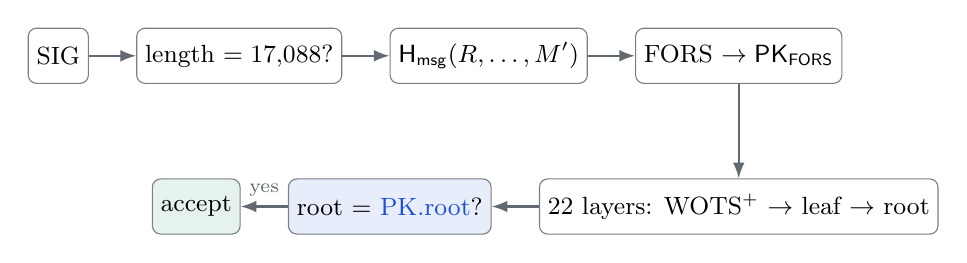
\begin{tikzpicture}[node distance=5mm and 6mm]
    \node[box] (sig) {SIG};
    \node[box, right=of sig] (len) {length $=17{,}088$?};
    \node[box, right=of len] (dg) {$\mathsf{H_{msg}}(R, \ldots, M')$};
    \node[box, right=of dg] (fp) {FORS $\to \mathsf{PK}_{\mathsf{FORS}}$};
    \node[box, below=12mm of fp] (ht) {22 layers: WOTS$^+$ $\to$ leaf $\to$ root};
    \node[box, left=of ht, fill=pub!10] (cmp) {root $=$ \pk{PK.root}?};
    \node[box, left=of cmp, fill=sig!10] (ok) {accept};
    \draw[arr] (sig) -- (len); \draw[arr] (len) -- (dg); \draw[arr] (dg) -- (fp); \draw[arr] (fp) -- (ht);
    \draw[arr] (ht) -- (cmp); \draw[arr] (cmp) -- node[above, font=\scriptsize]{yes} (ok);
  \end{tikzpicture}
  \vspace{4mm}

  \small
  The verifier never learns a secret and never checks an intermediate value. It recomputes one path from the signature up to the root, and accepts only if that path ends at \pk{PK.root}.
  Every step reuses a function from signing: \texttt{fors\_pkFromSig}, \texttt{wots\_pkFromSig}, \texttt{xmss\_pkFromSig}.
\end{frame}

\begin{frame}{Step V1: parse, re-encode, re-hash \alg{20, lines 1--13}}
  \begin{enumerate}
    \item Reject unless $|\mathsf{SIG}| = (1 + k(1+a) + h + d\cdot\mathit{len})\cdot n = 17{,}088$.
    \item Split: $\sg{R}$ = bytes 0--15, $\sg{\mathsf{SIG_{FORS}}}$ = 16--3,711, $\sg{\mathsf{SIG_{HT}}}$ = 3,712--17,087.
    \item Rebuild $M' = \hx{00} \cat |\mathit{ctx}| \cat \mathit{ctx} \cat M$ with the verifier's own context.
    \item $\mathit{digest} = \mathsf{H_{msg}}(\sg{R}, \pk{\mathsf{PK.seed}}, \pk{\mathsf{PK.root}}, M')$ and split it exactly as in Step 4.
  \end{enumerate}
  \vspace{2mm}
  \begin{block}{Example: the verifier gets the signer's values back}
    \small $\mathit{md} = \hx{4ecb\ldots82f0}$,\quad $\mathit{idx}_{\mathit{tree}} = 6541722705861835079$,\quad $\mathit{idx}_{\mathit{leaf}} = 1$,\quad indices $19, 44, 45, \ldots$
  \end{block}
  \small A changed message or context gives a different digest, hence different indices and a different tree path, and the final root comparison fails.
\end{frame}

\begin{frame}{Step V2: FORS public key from the signature \alg{17}}
  For each tree $i$ with index $t = \mathit{indices}[i]$:
  \begin{enumerate}
    \item $\mathit{node} \gets \mathsf{F}(\pk{\mathsf{PK.seed}}, \mathsf{ADRS}_{\text{height }0,\ \text{index } i\cdot 2^a + t}, \sg{\mathit{sk}_i})$
    \item For $j = 0, \ldots, a-1$: if bit $j$ of $t$ is 0, $\mathit{node} \gets \mathsf{H}(\mathit{node} \cat \sg{\mathit{auth}_j})$; else $\mathit{node} \gets \mathsf{H}(\sg{\mathit{auth}_j} \cat \mathit{node})$. Halve the tree index each level.
    \item $\mathit{root}_i \gets \mathit{node}$
  \end{enumerate}
  Then $\mathsf{PK}_{\mathsf{FORS}} = \mathsf{T}_k(\ldots, \mathit{root}_0 \cat \cdots \cat \mathit{root}_{32})$.
  \vspace{2mm}
  \begin{block}{Example}
    \small Tree 0, $t = 19 = 010011_2$. Reading bits from the lowest: $1,1,0,0,1,0$, so the running node is a right child at levels 0, 1 and 4 and a left child at levels 2, 3 and 5.\\
    Result: $\mathsf{PK}_{\mathsf{FORS}} = \hx{0608a9a55575d3e4ed2b4b692f07fd67}$, the same value the signer computed.
  \end{block}
  \small\textcolor{quiet}{Cost: $33 \times (1 + 6) + 1 = 232$ hash calls.}
\end{frame}

\begin{frame}{Step V3: WOTS$^+$ public key from the signature \alg{8}}
  \begin{enumerate}
    \item Recompute the 35 digits of the signed message (here \pk{$\mathsf{PK}_{\mathsf{FORS}}$}), checksum included.
    \item Continue chain $i$ from the signature value for the remaining $15 - \mathit{msg}[i]$ steps (hash addresses $\mathit{msg}[i], \ldots, 14$).
    \item Compress the 35 chain ends: $\mathit{leaf} = \mathsf{T}_{35}(\pk{\mathsf{PK.seed}}, \mathsf{ADRS_{WOTS\_PK}}, \ldots)$.
  \end{enumerate}
  \vspace{2mm}
  \begin{block}{Example, layer 0}
    \small Digits \hx{0 6 0 8 10 9 \ldots\ 6 7 | 0 15 1}: chain 0 needs 15 more steps, chain 1 needs 9, \ldots, chain 34 needs 14.\\
    Steps over all 35 chains: $35 \cdot 15 - (239 + 0 + 15 + 1) = 270$ F calls.
  \end{block}
  \small If the signature value was not on the chain, or the digits changed, the end value differs, and so does every hash above it.
\end{frame}

\begin{frame}{Step V4: climb each XMSS tree \alg{11}}
  \begin{columns}[c]
    \column{0.46\textwidth}
    \centering
    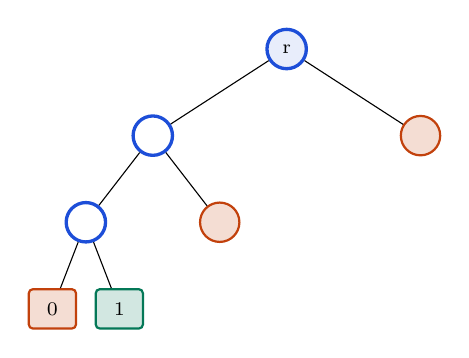
\begin{tikzpicture}[level distance=11mm, every node/.style={node},
        level 1/.style={sibling distance=34mm}, level 2/.style={sibling distance=17mm},
        level 3/.style={sibling distance=8.5mm}]
      \node[path, fill=pub!10] {r}
        child {node[path] {}
          child {node[path] {} child {node[leaf, au] {0}} child {node[leaf, hl] {1}} }
          child {node[au] {} } }
        child {node[au] {} };
    \end{tikzpicture}\\
    \footnotesize\textcolor{quiet}{Leaf 1 of layer 0: $1 = 001_2$.}
    \column{0.52\textwidth}\small
    Start at the recomputed WOTS$^+$ leaf, then for $k = 0, 1, 2$:
    \begin{itemize}
      \item bit $k$ of $\mathit{idx}$ is 1 $\Rightarrow$ $\mathsf{H}(\sg{\mathit{auth}_k} \cat \mathit{node})$ (we are a right child)
      \item bit $k$ is 0 $\Rightarrow$ $\mathsf{H}(\mathit{node} \cat \sg{\mathit{auth}_k})$
    \end{itemize}
    Leaf 1: right, then left, then left.\\[2mm]
    The address carries layer $j$, tree $\mathit{idx}_{\mathit{tree}}$, height $k+1$ and the node index. A node from another tree or layer cannot be substituted.
  \end{columns}
\end{frame}

\begin{frame}{Step V5: up the hypertree to \pk{PK.root} \alg{13}}
  \begin{columns}[T]
    \column{0.55\textwidth}
    \centering\footnotesize
    \begin{tabular}{@{}r r r l@{}}
      \toprule
      layer & tree & leaf & recomputed root \\
      \midrule
      0 & 6541722705861835079 & 1 & \hx{f53a8878df9fe723\ldots} \\
      1 & 817715338232729384 & 7 & \hx{8408b49a824b09b1\ldots} \\
      2 & 102214417279091173 & 0 & \hx{a3076cb6f98fa795\ldots} \\
      3 & 12776802159886396 & 5 & \hx{08d99af157ae0ccf\ldots} \\
      $\vdots$ & & & \\
      20 & 5 & 5 & \hx{5aa239e1b15208af\ldots} \\
      21 & 0 & 5 & \textbf{\hx{a90e4715b9a925c3\ldots}} \\
      \bottomrule
    \end{tabular}
    \column{0.42\textwidth}\small
    \begin{itemize}
      \item Each layer's root is the message for the next layer's WOTS$^+$ signature.
      \item After layer 21 the result is compared with \pk{PK.root}:\\[1mm]
        \hx{a90e4715b9a925c3}\\\hx{32801767fd786371}\quad \textcolor{sig}{\textbf{equal: accept}}
      \item This is the only comparison in verification. Its inputs are public, so it need not be constant time.
    \end{itemize}
  \end{columns}
\end{frame}

\begin{frame}{Why a forgery fails}
  \begin{itemize}
    \item \textbf{Change $M$ or $\mathit{ctx}$:} new digest $\Rightarrow$ new FORS indices and tree position. The forger needs leaf secrets that were never revealed, or a second preimage of $\mathsf{H_{msg}}$.
    \item \textbf{Change a FORS element:} its root changes $\Rightarrow$ PK$_{\text{FORS}}$ changes $\Rightarrow$ the WOTS$^+$ chains end at the wrong values.
    \item \textbf{Change a WOTS$^+$ element:} pushing a chain forward breaks its end value; going backward requires inverting F. The checksum blocks raising digits.
    \item \textbf{Swap an authentication node:} its address encodes layer, tree, height and index, so nodes do not transplant.
  \end{itemize}
  \vspace{2mm}
  \small\textcolor{quiet}{Security rests only on properties of the hash function. Each key may sign up to $2^{64}$ messages (FIPS 205 Section 11).}
\end{frame}

% ================================================================ wrap-up
\begin{frame}{What changes in the other parameter sets}
  \small
  \begin{tabular}{@{}>{\raggedright\arraybackslash}p{4.4cm} >{\raggedright\arraybackslash}p{9.6cm}@{}}
    \toprule
    Variation & Effect on the steps \\
    \midrule
    ``s'' sets ($h'=8$--$9$, $a=12$--$14$) & Same steps; fewer layers, taller trees: slow signing, small signatures \\
    $n = 24, 32$ (categories 3, 5) & Longer nodes; $\mathit{len} = 51, 67$ chains \\
    SHA2 instantiation & 22-byte compressed ADRS; PK.seed padded to one block; HMAC and MGF1 \\
    SHA2, categories 3 and 5 & H, T$_\ell$, PRF$_{\text{msg}}$, H$_{\text{msg}}$ use SHA-512; PRF and F stay SHA-256 \\
    256f ($h - h' = 64$) & $\mathit{idx}_{\mathit{tree}}$ uses all 64 bits: mask with care \\
    Pre-hash (HashSLH-DSA) & $M' = \hx{01} \cat |\mathit{ctx}| \cat \mathit{ctx} \cat \mathsf{OID} \cat \mathsf{PH}(M)$; the rest is identical \\
    \bottomrule
  \end{tabular}
\end{frame}

\begin{frame}{Summary}
  \begin{columns}[T]
    \column{0.48\textwidth}
    \textbf{Signing}
    \begin{enumerate}\small
      \item $M'$ from message and context
      \item $R = \mathsf{PRF_{msg}}$ (hedged or deterministic)
      \item $\mathit{digest} = \mathsf{H_{msg}}$
      \item split: $\mathit{md}$, $\mathit{idx}_{\mathit{tree}}$, $\mathit{idx}_{\mathit{leaf}}$
      \item FORS: reveal $k$ leaves and their auth paths
      \item hypertree: $d$ WOTS$^+$ signatures with auth paths
      \item $\mathsf{SIG} = R \cat \mathsf{SIG_{FORS}} \cat \mathsf{SIG_{HT}}$
    \end{enumerate}
    \column{0.48\textwidth}
    \textbf{Verification}
    \begin{enumerate}\small
      \item check the length, split
      \item recompute the digest and its split
      \item FORS leaves $\to$ roots $\to$ PK$_{\text{FORS}}$
      \item per layer: finish chains $\to$ leaf $\to$ root
      \item accept iff the last root $=$ PK.root
    \end{enumerate}
    \vspace{3mm}
    \footnotesize
    \textbf{Reproduce every number:}\\
    \texttt{cargo run --example running\_example}\\
    \texttt{python3 docs/slides/trace.py \ldots}\\[2mm]
    \textbf{References:} NIST FIPS 205 (2024); github.com/V-k-h/slhsig
  \end{columns}
\end{frame}

\end{document}
